\chapter{Discussion}
\label{chapter:evaluation}

%You have done your work, but that's\footnote{By the way, do \emph{not} use
%shorthands like this in your text! It is not professional! Always write out all
%the words: ``that is''.} not enough. 

%You also need to evaluate how well your implementation works.  The
%nature of the evaluation depends on your problem, your method, and
%your implementation that are all described in the thesis before this
%chapter.  If you have created a program for exact-text matching, then
%you measure how long it takes for your implementation to search for
%different patterns, and compare it against the implementation that was
%used before.  If you have designed a process for managing software
%projects, you perhaps interview people working with a waterfall-style
%management process, have them adapt your management process, and
%interview them again after they have worked with your process for some
%time. See what's changed.

%The important thing is that you can evaluate your success somehow.
%Remember that you do not have to succeed in making something spectacular; a
%total implementation failure may still give grounds for a very good master's
%thesis---if you can analyze what went wrong and what should have been
%done. 

 %At this point, you will have some insightful thoughts on your
%implementation and you may have ideas on what could be done in the
%future. This chapter may be combined together with the evaluation
%chapter. All the new insights and findings are given here!  This
%chapter is a good place to discuss your thesis as a whole and to show
%your professor that you have really understood some non-trivial
%aspects of the methods you used\ldots

In this final chapter before conclusion, we will be evaluating our methology through the pipeline that was build in the previous chapter.
We will be using the qualitive metrics that we defined in the planning chapter before implementation.
Finally, we end this chapter by contemplating on how this pipeline and process could improved in the future.

\section{Method evaluation}

%In this section we will be focusing on the three metrics we introduced previously.
We have divided this evaluation strictly to advantages and disadvantages, and we will be using the metrics that we depicted in the methology chapter.
We have summarized these in the figure 6.1 and we will be opening up these in the following sections.
We will be comparing our way of building the pipeline with the two somewhat similar existing pipelines to see which are the advantages and disadvantages of using one for novice data scientist.

\begin{table}[! htbp]\centering 
  \caption{Advatanges and disadvantages of the methology}
  \begin{threeparttable}
      \begin{tabular}{|p{6cm}|p{6cm}|}
      \hline
      Advantages & Disadvantages \\ \hline
      Cost efficient & No promises on scaling/Runs only on one hardware \\ 
      Sustainable & Docker introduces more complexity \\ 
      Easy to reproduce & \\ \hline
      \end{tabular}
  \end{threeparttable}
\end{table}

\subsection{Advantages}

Let us start with the most obvious advantage of using this method: it is very cost efficient when it comes to running the pipeline.
No cloud subscription or local cluster is needed to run and test the pipeline.
As we saw in the previous chapter, this methology does not erase the problems that arise integrating the technologies, but using it does erase the cost of debugging this against cloud platform where every run of the program costs money.
We cannot make direct comparisons with academic pipeline as we do not have exact information on if the pipeline is run on a local cluster but we can say that the pipeline is much more cheaper than the industrial pipeline.

The sustainability of the pipeline is also an advantage in this case.
Compared to the local academic pipeline, where each components version has to be manually confirmed when it is installed and updating components means that everyone who wants to run newer versions of the pipeline has to do the same, our version does not suffer from these problems as these are defined in the docker configuration files.
Compared to the industrial pipeline, however, the process is probably taken into step further as Amazon can keep the components better up to date by automatically updating minor versions, which our current methods do not necessarily do.
Of course, this depends a lot on the docker image provider and their methology on versioning, but in our example case this seemed to provide efficient way to handle versioning.

The reproducibility of the pipeline is an another advantage.
Using docker and docker compose to build the pipeline we were able to limit the number of external dependencies to only these two when a new user wants to run the pipeline and with only couple minor exceptions we were able to automate the local setting up process.
Also the usage of Zeppelin notebooks allows the user to share their models with anybody who has the same pipeline or other means to run them.
When we compare this to the academic pipeline which had all of its components as local dependencies, the amount of possible work is greatly smaller as the user does not have to install each component to their local machine and worry about their versions.
As what comes to the automation of the setting up the pipeline, we have no information on this to make any reasonable claims.
When compared to the industrial pipeline, although not reported, we can pretty much assume that the industrial pipeline is highly reproducible as there are probably ten to hundred employees working with the pipeline and in this sense is probably a lot more reproducible than the pipeline presented here.
This could be due to inherent nature of containarized applications in AWS and the tooling that continuous integration tools and Amazon provide.

\subsection{Disadvantages}

For the disadvantages, clearly, our pipeline has only run on one machine and we still have no proves that it would scale to big data order of magnitude.
Compared to the industrial pipeline we can clearly state that our pipeline does not yield same kind of efficiency as a pipeline run on cloud.
This is a clear disadvantage of this methology.

Related to this is the inherent nature of running the pipeline only on one machine.
The virtual distributed environment does allow us to simulate networks that are needed to configure the system, but the underlying hardware does not allow us test it with an amount of data that is too much for one machine.

Adding docker to the mix of technologies does bring a bit more complexity to the system.
As we saw in the previous chapter this can introduce quite challenging problems when trying to integrate these technologies together.


%Currently the de facto way to train machine learning models is to use graphics cards as they provide tremendously better perfomance when compared to CPUs.
%Our pipeline build with this method, however, does not inherently support this.
%So the amount of computers needed to run the training on this pipeline is greatly larger if we wanted to produce same perfomance as even single-machine GPU provides. 

%\subsection{Reproducibility}

%As stated before, in this characteristic we will be focusing on how much manual work must the user do in order to run the pipeline.
%Using docker and docker compose to build the pipeline we were able to limit the number of external dependencies to only these two when a new user wants to run the pipeline and with only couple minor exceptions we were able to automate the local setting up process.
%Also the usage of zeppelin notebooks allows the user to share their models with anybody who has the same pipeline or other means to run them.

%When we compare this to the academic pipeline which had all of its components as local dependencies, the amount of possible work is greatly smaller as the user does not have to install each component to their local machine and worry about their versions.
%As what comes to the automation of the setting up the pipeline, we have no information on this to make any reasonable claims.

%When compared to the industrial pipeline, although not reported, we can pretty much assume that the industrial pipeline is highly reproducible as there are probably ten to hundred employees working with the pipeline and in this sense is probably a lot more reproducible than the pipeline presented here.
%This could be due to inherent nature of containarized applications in AWS and the tooling that continuous integration tools and Amazon provide.

%\subsection{Sustainability}

%Compared to the local academic pipeline, where each components version has to be manually confirmed when it is installed and updating components means that everyone who wants to run newer versions of the pipeline has to do the same, our version does not suffer from these problems as these are defined in the docker configuration files.
%Compared to the industrial pipeline, however, the process is probably taken into step further as amazon can keep the components better up to date by automatically updating minor versions, which our current methods do not necessarily do.
%This depends a lot on the docker image provider and their methology on versioning.


%\subsection{Novice friendliness}

%With our choices on docker and scala we have achieved somewhat easier pipeline to handle for novices.
%With Docker it was possible to abstract away a lot of the complexity which there was to run the different components.
%This of course increased the amount of work to build the pipeline but once it was built it could be run without any knowledge on underlying system.

%The choice of Scala was reasoned because of its interoperativity with spark and support for multiple paradigms.
%It also ran over JVM which made it easier to justify it as all the other technologies ran too.
%However as seen with the challenges in the previous chapter, somewhat better choice for novices could have been Python.
%Both of these languages are taught as beginner languages in Aalto University, but Python might have had better support for deep learning models although integrating this with Spark would have probably still introduced challenges.

%When compared to the academic pipeline, the amount of work to build this first time, was probably greater than with the academic pipeline because Docker brought one more component to integrate with every other component.
%This could be seen in the challenges faced that we examined in the previous chapter.

%Compared to the industrial pipeline, with the help of docker we were able to make the pipeline easy to run locally in a virtually distributed setting without spending any money.
%This can be very crucial difference because as stated before, our target group definitely does not have as much resources than the company running the reference industrial pipeline.

%\section{Reflecting challenges}

%Next we question, whetever the challenges faced during development were significant in the sense that they could actually cause harm to novice data scientists.

%With the Kafka-HDFS integration we can argue that the necessary information was available online and anyone looking to build the integration could have found this with little to none research, which is absolutely correct.
%From the ocean of possible alternatives, we could have found other solutions also such as Flume which some were suggesting.
%This is not the worst kind of problem there is as the information, although scattered, is available in the internet.
%The actual problem here is that because there is no clear consensus on what to use and what are the advantages and disadvantages over another, the process of picking right technology can be very stressful.
%What can be said about implementing this integration itself is that we can critize our solution to run it outside Confluent environment making the environment itself non-friendly for novices, in which case the lack of documentation is only a problem caused by ourselves to ourselves, which is true.

%With the Zeppelin dependency management problems the real problems started.
%Instead of giving easy to understand way to handle the dependency errors, user is mostly left with learning maven dependency management which is hidden inside the zeppelin itself.
%Probably the best solution would have been to build the service on top of docker from ground up.
%This, however, is far from novice friendly way to use the component as it needs a lot of external knowledge to produce a valid setup which is why the usage of the software itself becomes very hard for novices.

%The DL4J with Scala using sbt, the major thing here to be questioned is the choice of sbt.
%As there was no up to date DL4J project with sbt we can make a conclusion that sbt is not relevant in this field.
%sbt, however, is the most well known build tool for Scala so if a library has a scala support it would not be far fetched to hope a working up to date example of this as most novices really do need them as reference to build their own applications.

%Finally we had the problem with running the DL4J on a docker based Spark instance with Zeppelin.
%This as a combination is definitely not the combination that probably any of the singular component makers probably thought which is reasonable as there are so many possible options.
%This highlights well the challenges that come from having so many different possible options that are recommended by themselves without context.
%One can question whetever we did caused this to ourselves and as the stack can be thought very exotic the blame is all ours in this sense, but given the reasoning we used for each choice in this stack, we think that is reasonable to assume that this could happen anyone with the same kind of requirements.
%Of course a lot of this could have been avoided if Scala was replaced for example with Python but these are assumptions we cannot prove to be wrong or right.

\section{Future improvements}

The lack of reference points made it hard to compare this way of building a pipeline with other possible ways.
Hopefully in the future, the information about these systems would become more open so that we could better understand them, but until then we have to work with what we have.
The use of only one example is also a clear point of improvement as it does not prove much about the functionality of our methology.
More specific cases would be needed to make more believable deductions.

For the methology itself, better instructions on how to deploy the pipeline to the cloud would have probably solved a lot of disadvantages that we saw in the previous section.
Also a better instructions on running the pipeline in distributed GPU environment would have probably greatly improved the efficiency of model training.
Unfortunately due to lack of time this was not possible, but would be a great way to improve the information here as there is not that many examples online of this kind of process.


%\section{Perfomance metrics}

%We start by defining the environment where the following results were derived.
%The following metrics were taken in a machine that has a Windows 10 as parent operating system, Intel Core i5 2500K processor and 16GB of DDR3 memory.
%The docker version that the code was run against was 19.03.2 and it had 3 CPU cores and 10GB of memory as its use.
%Not all of these resources were needed, but this was done to in order to remove the factors of running out of memory that could cause inexplicable errors.
%These were tested only in one machine which would usually not be enough to make any kind of actual inferences but because the code is run in a containerized environment the role of underlying hardware becomes less important.

%\begin{figure}[ht!]
%    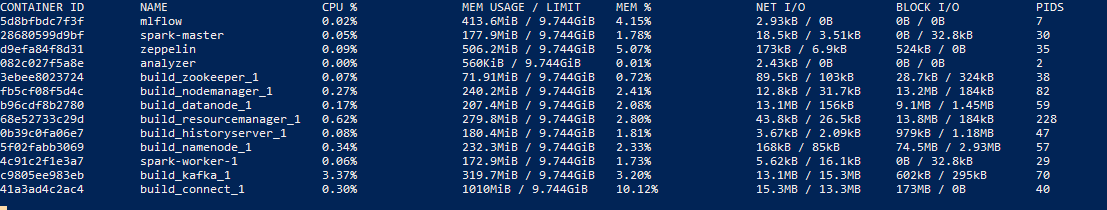
\includegraphics[scale=0.45]{images/memory1} 
%    \centering
%    \caption{Resource usage in idle state}
%\end{figure}

%The resource usage in idle state after the initial data has gone through the pipeline and stored into HDFS can be seen in the figure 6.1.
%The figure is the output of the "docker stats" -command.
%While inspecting the names of each container the reader should be able to map these into corresponding components in the architechture figure in section 5.2, but to clarify the most ambigous namings, the "analyzer" container refers to the standalone DL4J application and build\_connect\_1 refers to the Kafka Connect instance.

%The total memory usage here was around 3.8GiB.
%This seems to match with the fact that most of the components ran on top JVM and we did not have the time to optimize each components garbage collection. 
%This is partly because components such as the Kafka Connect, which had a notably large memory usage, would silently fail if not enough memory were offered.
%Additionally, this would have probably lead to premature optimization.
%For future improvements on the accessibility of the pipeline, this would be a great place to start.

%Processor usage in idle state was minimal and did not have any notable jumps except a bit higher usage for Kafka.
%The other statistics did not have any notable deviations that would affect greatly on the usage of the pipeline. 
%Minor thing to note is that the DL4J application instance is not running actively during these results as user usually are not using both it and the zeppelin instances simultaneously.

%\begin{figure}[ht!]
%    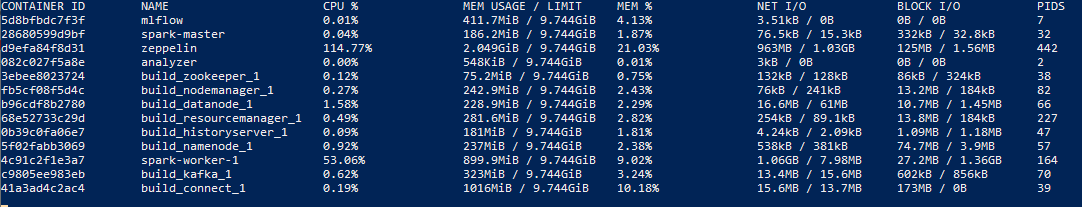
\includegraphics[scale=0.45]{images/memory2} 
%    \centering
%    \caption{Resource usage in preprocessing state}
%\end{figure}

%In figure 6.2 we have the same statistics while the zeppelin code is trying to preprocess the data in order to feed it into LSTM network.
%The pipeline has at this point run for some time and the overall memory load has increased to 6.1GiB.
%This is mainly due to Zeppelin and Spark worker using a lot more memory.
%The CPU usage for both has raised, and one can see that at the moment of taking these stats the notebook code is actually using more resources than the actual worker.

%As there was not enough time to test other technologies in pipeline these results by themselves do not give us much information about the quality of the software.
%They do give us some information about the requirements of the machine that is needed to run locally a pipeline that is this complex.
%Over 8GiB of memory is almost a must to run it in active use where the data is flowing continously.
%The need for memory can be alleviated with proper garbage collection, but peak memory usage can reach to these numbers.

%\section{Pipeline management}

%The main benefits of this pipeline do not come from its perfomance.
%It is highly containerized meaning it can run with little to none re-configuration on any machine.
%During the development of this pipeline the pipeline was developed first on Mac OS and then because of memory requirements moved to Windows machine.
%The porting of code did not require any extra steps, other than making sure that the formating of line endings stayed the same with script files that are run in containerized linux environment.

%Docker containers also allow the development in isolated networked environment that is very similar to one which would be used in production.
%This means that most of the problems that could occur when rolling locally developed code into a production environment where services lie on different machine interconnected by a network, are already solved in here before the user has even started development.
%Only thing that the user has to do is to change the addresses in this code from docker based DNS to the addresses used in their own cloud environment.

%As explained earlier, the technologies such as Kafka Connect have been chosen so that changing one techonology does not have large impacts on the overall architecture.
%If the user would want to change some component in the pipeline, the integrations between components have to be done again but this has been made as easy as possible.

%The pipeline is also mostly automated.
%No manual input is required from the user to setup the basic pipeline which makes adapting the pipeline quite trivial.
%Only in the analysis phase, users manual input is needed to control the pipeline.

%Machine Learning pipeline monitoring is made easy with MLFlow.
%Although logging new experiments needs a bit of manual work for user because of the nature of MLFlow API, but nevertheless it does make managing the machine learning models easier.
%The only downside here is that by default MLFlow does not yet accept DL4J models to be saved in its containerized packages which would make model export easier.

%For general monitoring the pipeline is still lacking because we did not have time to implement the ELK stack.
%Almost each component has its own monitoring UI but these are scattered making it hard to follow the bigger picture of the pipeline which was one of the problems we introduced in the chapter 2.
%The exception of not having an own monitoring UI is the Kafka Connect.
%It offers REST API to monitor its metrics which would need additional integration with some log monitoring solution such as ELK.

%\section{Flaws in the end product}

%In this section we examine general flaws in the pipeline that we are aware of.
%We try to objectively examine these and try to give some reasoning why these flaws did happen and how they could be fixed.
%We will leave out here the flaws in monitoring as these were mostly examined in the previous section.

%Currently, the main method of training machine learning models is to use computers graphics card (GPU) which is multiple times faster than using CPUs.
%This makes the current pipeline vastly underperforming when it comes to training machine learning models and this is a clear downside for this system.
%It needs quite a bit of CPUs and good networking before it even reaches the perfomance of a single high-end GPU.
%The DL4J, does however, support GPU training on spark cluster meaning that adding GPU support to this pipeline with small amount of work is possible.
%However, we did not have time to implement it as it needs some work for docker to access CUDA resources on parent OS.

%Unfortunately, because we were only able to try the HDFS as the storage method, the storage is currently lacking a proper query properties meaning that the user has to pull the entire timeseries for each stock.
%This in big data context is not desirable behaviour, but integrating a technology like HBase should not need much additional work.
%However, for us it is already out of the scope of this project.

%With the resources this project had, the pipeline could not be tested with actual complete stock market data, which leaves means that we have no prove that the pipeline actually can scale with the data or if this scaling is even possible with the pipeline.
%We can only speculate this based on the each of technologies abilities but the possibility for horizontal scalability should be there theoretically.

%\section{Reflection}

%In this section we will reflect back on the implementation part and discuss what possibly went wrong on the development of the pipeline.
%We will try our best to explain the choices taken while being aware that there could have been better alternatives.

%Choosing DL4J as the machine learning library turned out to be a time consuming option.
%After the implementation part, it was clear why data scientist usually use python libraries such as Keras and PyTorch, the amount of resources is substantially larger.
%Many of the problems faced during development had quite simple solutions to them, but they were really hard to solve without any reference and empty search results on Google.
%This combined with the out-of-date examples lead to problems seen in the previous chapter.

%One can question whetever we should have opted out from DL4J during development and changed it to some other more compatible library.
%We did not do this because there was not that many sensible choices and the documentation and resources online of those that seemed promising were even worse than with the DL4J.
%But although the original plan to build to multiple pipelines was not possible partly because of this, we think that the information produced in the implementation chapter is quite valuable on its own and can help a lot of novice data scientists who have restrictions on what technologies they can use.

%Of course, the scope of the implementation part could have been narrowed down as it was quite ambigous.
%Especially, during development things that seemed simple turned out to be quite more complex than initially thought.
%The inexperience about some of the technologies used did affect the results, but it also indicates that the documentation of some technologies could have been better.
%Quite a bit of things were assumed in the documentations, which lead to errors that probably could not had happened with right documentation.

%\section{Potential improvements}

%There are quite a bit of improvements already mentioned at the previous sections as these usually are part of the problems, but we have gathered them and a couple others to this section to give a clearer view on what could be improved.
%These are quite straightforward to implement but implementing them can take some time.

%As stated before, the perfomance of the pipeline could be improved.
%This could be done by adding support for GPU usage in Spark cluster which would require the configuration of docker to give the process access to these.
%Memory usage could be probably optimized by configuring better carbage collection on components that take most of the memory.

%To make the pipeline more automated and improve its mobility, urls for servers could be made dynamic with for example environmental variables that could be configured by the user.
%Other such configurations could be made in order to make porting the code to a different environment easier.

%The final giveaway in this chapter is that there was quite a bit of things that could have been done better. 
%This is partly because of the ambigious scope of the project, inexperience of the author and lack of correct information online.
%Despite these, we think that the complications during the development and the final product do offer valuable insights on developing a pipeline for stock data analysis using these technologies and can give somebody a basis to start developing their own pipeline.
%Now we move on to the final chapter where we conclude and summarize everything that we have learned during this thesis.